\cotefile{29}
\scanpage{141}
$S$ \deleted{\unsure{$/$}} préschéma connexe \uline{réduit}

\deleted{\unsure{$\mathscr{G}$ catégorie de groupes}

$\mathscr{C}$ une catégorie auxiliaire

$\mathscr{G}$ ss-catégorie pleine de $\mathrm{Gr}(\mathscr{C})$}

\diagram{\begin{tikzcd}[ampersand replacement=\&]
\bar G \arrow[r,"{(u,v)}"] \& \bar G'\times\bar G' \\
\bar H \arrow[u]\arrow[r] \& \bar G'\arrow[u]
\end{tikzcd}}

\diagram{\begin{tikzcd}[ampersand replacement=\&,column sep=small]
(P,\xi)\arrow[r] \& (Q,\eta)=(P,\xi)\times_G\unsure{(G'\times G')}\\
(R,\lambda)\arrow[u]\arrow[r] \& (P',\xi')\arrow[u]
\end{tikzcd}}

$\mathscr{C}$ une catégorie de $S$-groupes \uline{finis} et \uline{plats}

$\mathscr{C}$ stable par produits, \deleted{et} par \uline{noyaux} \deleted{\unsure{plats}} de couples de morphismes, par \uline{images}

Les $G\in\mathscr{C}$ sont \uline{admissibles}.

On \deleted{définit} suppose $S$ \uline{pointé} par $a$,

Si $G\in\mathscr{C}$, on pose $\unsure{\mathfrak{Z}|\mathfrak{F}}(G)=\mathfrak{Z}(S,a;G)={}$ classes de fibrés \inserted{homog.} principaux $a$-pointés de groupe $G$

Éléments minimaux de $\mathfrak{Z}(G)$.

\uline{Proposition 4} Soit $\alpha\in\mathfrak{Z}(G)$ minimale. Alors $u\mapsto u_*(\alpha)$ de $\mathrm{Hom}^{\mathrm{gr}}_S(G,G')$ dans $\mathfrak{Z}(\unsure{G'|Q'})$ est \uline{injectif} \hfill $[G,G'\in\mathscr{C}]$

$u,v\in\mathrm{Hom}^{\mathrm{gr}}_S(G,G')$ tels que \deleted{\unsure{$u_*(\alpha)=v_*($}} $u_*(\alpha)=v_*(\alpha)$.

$(P,\xi)$ de classe $\alpha$, $(P',\xi')$ de classe $u_*(\alpha)=v_*(\alpha)$,

\[
(u,v):G\longrightarrow G'\times G',\quad \text{et}\quad
(Q,\eta)=(P,\xi)\mathop{\times}_{G}(G'\times G')
=\big[(P,\xi)\mathop{\times}_{u}G'\big]\times\big[(P,\xi)\mathop{\times}_{v}G'\big]
\]

Par hypothèse, on a un hom. \inserted{(d'ailleurs \uline{unique})} $(P',\xi')\longrightarrow(Q,\eta)$ compatible avec $G'\xrightarrow{\mathrm{diag}}G'\times G'$, Soit $(R,\lambda)$ le produit fibré de $(P,\xi)$ et $(P',\xi')$ sur $(Q,\eta)$. \deleted{Soit $Z$ un $S$-schéma, on} \inserted{Soit $H$ le noyau de} $G\overset{u}{\underset{v}{\rightrightarrows}}G'$, je dis que $(R,\lambda)$ \uline{est un fibré pr. hom. pointé sous $H$} [ et \unsure{de|la} condition \unsure{minimal|minimale} de $(P,\xi)$ résultera \unsure{donc|alors} que $H=G$, d'où $u=v$ ]. En effet, il suffit de \deleted{\unsure{le}}\unsure{vérifier|montrer} \deleted{\unsure{localement}} en faisant l'extension de base $(S_1,a_1)=(P,\xi)\longrightarrow(S,a)$, ce qui nous \unsure{ramène|simplifie|à remplacer}

\margin{$S\leftarrow S_1$}

\margin{\deleted{\unsure{$g\,g$}}\\ $u(g)=g'$\\ $v(g)=g'_1g'$\\ $u(g)=g_1'^{-1}v(g)$}

% archive sheet number: 140

\scanpage{142}
la situation pour $G_1$, $G'_1$, $(P_1,\xi_1)$, $(Q_1,\eta_1)$ etc. [Attention, on perd le fait que $\unsure{S_2|S|S_1|Q_1}$ soit réduit, $S_1$ ne l'étant plus]. $P_1$ s'\uline{identifie} alors $G_1$\inserted{(muni du \unsure{pt distingué|point marqué|marquage} $\varepsilon_1$)}, $Q_1$ à $G'_1\times_{S_1}G'_1$ muni de $(\varepsilon'_1,\varepsilon'_1)$, \deleted{je dis que} enfin $(P'_1,\xi'_1)$ s'identifie aussi à $(G'_1,\varepsilon'_1)$. Il suffit de voir que $(P'_1,\xi'_1)\to(\unsure{Q'_1|Q_1},\eta_1)$ est l'application diagonale $G'_1\unsure{-|\to}G'_1\times_{S_1}G'_1$.

\uline{Or} \unsure{remontons} les définitions, et désignons par $w$ l'isom. $(P,\xi)\times_u G'\longrightarrow(P,\xi)\times_vG'$, $w_1$ l'isom. déduit par extension de la base à $S_1$, notre assertion signifie que $w_1$ transforme la section ``naturelle'' de $P_1\times_{u_1}G'_1$ dans celle de $P_1\times_{v_1}G'_1$, i.e. qu'on a commutativité dans

\diagram{\begin{tikzcd}[ampersand replacement=\&,column sep=small]
P=S_1\arrow[r]\arrow[rr,bend right=16] \& (P\times_uG')\times_S S_1\arrow[r,"{w_1=w\times_{\unsure{S|S,S}} S'}"] \& (P\times_v G')\times_S S_1
\end{tikzcd}}

ou encore qu'on a commutativité de

\diagram{\begin{tikzcd}[ampersand replacement=\&]
P\arrow[r,"\mathrm{can}"]\arrow[rr,bend right=15,"\mathrm{can}"']\& P\times_uG'\arrow[r,"w"]\& P\times_vG'
\end{tikzcd}}

\uline{Or cela résulte} de \uline{l'unicité} de $P\longrightarrow P\times_vG'$ \uline{transformant} \deleted{\unsure{$\xi$ en $\xi'$}} pt marqué en pt marqué \ldots.

% archive sheet number: 141

\scanpage{143}
\deleted{Ceci \unsure{prouvé|posé}}

D'autre part on a

\[
\unsure{\mathfrak{Z}|\mathfrak{F}|\mathfrak{z}}(G\times G')=\mathfrak{Z}(G)\times\mathfrak{Z}(G')
\]

et \deleted{\unsure{les}} l'ens. des sousgroupes $\in\mathscr C$ d'un $G\in\mathscr C$ satisfait la condition minimale.

Ces propriétés formelles suffisent pour construire un \uline{pro-objet} de $\mathscr C$, \deleted{\unsure{au}} au moyen d'un système projectif \unsure{de épimorphismes|d'épimorphismes}, qu'on \deleted{\unsure{pe}} désignera par $\pi_1^{\mathscr C}(S,\xi)$.

\uline{Exemple I} $\mathscr C={}$ \unsure{cas des groupes|ens. des groupes} définis par \unsure{des|un|les} \unsure{groupes finis ordinaires|groupe fini ordinaire}. On retrouve le groupe fondamental.

\uline{Exple II} $S$ est un préschéma au dessus d'un corps $k$. $\mathscr C$ provient d'une catégorie $\mathscr C_0$ de $k$-groupes finis (par exemple \deleted{\unsure{ét--|tous}} les $k$-groupes finis --- ce qui \deleted{\unsure{est}} \inserted{semble} raisonnable surtout si $k$ sep. clos) stable par produits, noyaux de couples, images.

% archive sheet number: 142

\scanpage{144}
\unsure{Compléments|Compliments} SGA\\
1960

% archive sheet number: 143

\scanpage{145}
\[
\begin{aligned}
  &\pi' &&\pi''_\alpha &&\pi'''_\beta\\
S\quad &\text{\uuline{$S'$}} &&\deleted{\unsure{\beta}}\, S''\deleted{\unsure{{}_{\alpha}}} &&S'''
\end{aligned}
\]

\[
p_{ij}^{\alpha\beta}:\pi'''_\beta\longrightarrow\pi''_\alpha
\quad\text{si }\alpha=p_{ij}(\beta)\qquad
(ij)=\begin{cases}(1,2)\\(2,3)\\(1,3)\end{cases}
\]

\[
p_i^\alpha:\pi''_\alpha\unsure{-|\longrightarrow}\pi'\qquad
i=\begin{cases}1\\2\end{cases}
\]

\[
\deleted{\unsure{p_i^\alpha p_{ij}^{\alpha\beta}}}\quad
\left\{\begin{aligned}
 p_1^\alpha p_{12}^{\alpha\beta}&=\operatorname{int}(a'_\beta)p_1^\alpha p_{13}^{\alpha\beta}\\
 p_2^\alpha p_{12}^{\alpha\beta}&=\operatorname{int}(a''_\beta)p_1^\alpha p_{23}^{\alpha\beta}\\
 p_2^\alpha p_{13}^{\alpha\beta}&=\operatorname{int}(a'''_\beta)p_2 p_{23}
\end{aligned}\right.
\]

\[
\begin{aligned}
p_{12}^{-1}(p_1^{-1}(E))&\longrightarrow p_{12}^{-1}(p_2^{-1}(E))&
(p_1p_{12})^{-1}(E)&\longrightarrow(p_2p_{12})^{-1}(E)\\
p_{23}^{-1}(p_1^{-1}(E))&\unsure{-|\to}p_{23}^{-1}(p_2^{-1}(E))&
(p_1p_{23})^{-1}(E)&\longrightarrow(p_2p_{23})^{-1}(E)\\
p_{13}^{-1}(p_1^{-1}(E))&\longrightarrow p_{13}^{-1}(p_2^{-1}(E))&
(p_1p_{13})^{-1}(E)&\longrightarrow(p_2p_{13})^{-1}(E)
\end{aligned}
\]

\diagram{\begin{tikzcd}[ampersand replacement=\&,column sep=small]
(p_1p_{12})^{-1}(E)\arrow[r,"{\unsure{\wedge|\Lambda|A}}"]\arrow[d,"\wr"] \& (p_2p_{12})^{-1}(E)\arrow[r,"\sim"] \& (p_1p_{23})^{-1}(E)\arrow[d]\\
(p_1p_{13})^{-1}(E)\arrow[r] \& (p_2p_{13})^{-1}(E)\arrow[r,"\sim"] \& (p_2p_{23})^{-1}(E)\arrow[d,"{\deleted{\wr}}",description]\\
\&\& \deleted{(p_2p_{13})^{-1}(E)}
\end{tikzcd}}

Pour \unsure{tt|$\forall$} $\beta$, on doit avoir, posant $\alpha'=\underline{p_{12}(\beta)},\ \alpha''=p_{23}(\beta),\ \alpha'''=p_{13}(\beta)$, comm. de

\diagram{\begin{tikzcd}[ampersand replacement=\&]
E\arrow[r,"A_{\alpha'}"]\arrow[d,"{\wr\,a'_\beta}"] \& E\arrow[r,"{a''_\beta}","\sim" description] \& E\arrow[d,"A_{\alpha''}"]\\
E\arrow[r,"A_{\alpha'''}"] \& E\arrow[r,"{a'''_\beta}","\sim" description] \& E
\end{tikzcd}}

\[
\boxed{A_{\alpha''}a''_\beta A_{\alpha'}=a'''_\beta A_{\alpha'''}a'_\beta}
\]

% archive sheet number: 144

\scanpage{146}
\mspage{- 156 -}
\hfill n\textsuperscript{o} 280

\uline{Corollaire} - (Hilbert)- \uline{Soient} $k$ \uline{un corps}, $K$ \uline{une extension algébriquement close de} $k$, $P$ \uline{un} \uline{élément de} $B=k\,[X_1,\ldots,X_n]$, \uline{et} $n$ \uline{un idéal de} $B$. \uline{Les deux propriétés suivantes sont équivalentes} :

a) \uline{il existe un entier} $r$ \uline{tel que} $P^r\in n$ ;

b) \uline{pour tout $k$-homomorphisme} $f$ \uline{de} $B$ \uline{dans} $K$ \uline{tel que} $f(n)=\{0\}$, \uline{on a} $f(P)=0$.

En effet, $B$ est un anneau de Jacobson (Th.1) . Donc les polynomes de $B$ dont une puissance est dans $n$ sont ceux qui appartiennent à tout idéal maximal de $B$ contenant $n$ . Il suffit alors d'appliquer la prop.1c).

% archive sheet number: 145

\scanpage{147}
\deleted{Si on a choisi les $\bar s''$ et $\bar s'$ tels que \unsure{$\operatorname{diag}$} \inserted{\unsure{$s''=\operatorname{diag}_2(\bar s')$|$s'''=\operatorname{diag}_{\theta_2}(s'')$}} et \unsure{$s'''=\operatorname{diag}_3(\bar s')$|$s'''=\operatorname{diag}_{g_3}(s')$} \unsure{diag.|donc}.}

Il est loisible de supposer que pour \unsure{tt|$\forall$} $s'\in E'$, désignant par $s''$ et $s'''$ ses images dans $\unsure{E''',E'''|E'',E'''}$ par l'application diagonale, \deleted{on ait $\bar s''=\mathrm{diag}$.} $\unsure{\widetilde{\bar s}''|\bar s'''}$ sont les images de $\underline{\bar s'}$ et $\underline{\bar s''}$ par les morphismes diagonaux, et qu'on ait choisi \inserted{pour} les données \unsure{classes de chemins,|chemins de chemins,} \unsure{associées|associés} à ces $s'',s'''$ \deleted{les} les chemins triviaux. \inserted{(\unsure{Enfin}, on peut supp. que $s''=\bar s'$.)} Alors il résulte de $c$ qu'on a

\[
g_{s''}=g_{s''}g_{s''}\qquad\text{i.e.}\quad g_{s''}=1
\]

et \unsure{la relation|les relations} b) \unsure{prend|prennent|pour} la forme équivalente

\[
\tag*{b')}g_{\bar s'}=1.
\]

\figure{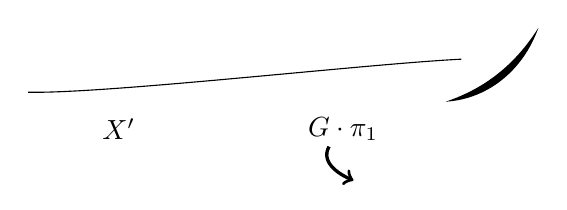
\begin{tikzpicture}[x=1cm,y=1cm]
\draw (0,0) .. controls (1,-.02) and (4.3,.36) .. (5.5,.42);
\fill (5.3,-.12) .. controls (5.75,.03) and (6.16,.31) .. (6.48,.82) .. controls (6.28,.26) and (5.82,-.09) .. (5.3,-.12);
\node at (1.15,-.47) {$X'$}; \node at (4,-.47) {$G\mathbin{\cdot}\pi_1$};
\draw[->,very thick] (3.82,-.69) .. controls (3.7,-.91) and (3.99,-1.06) .. (4.13,-1.12);
\end{tikzpicture}}

\[
S\longleftarrow S'
\]

\[
\begin{aligned}
&\pi\\[-2pt]
&\qquad\pi_1(\unsure{s'_1,a'|S',a'|S,\alpha})\quad\pi\qquad S
\end{aligned}
\]

\diagram{\begin{tikzcd}[ampersand replacement=\&,column sep=small]
\&R_0\arrow[d]\&R_1\arrow[d]\&R_2\arrow[d,shift left]\arrow[d]\arrow[d,shift right]\\
S\&S'\arrow[l]\&S''\arrow[l,shift left]\arrow[l,shift right]\&S'''\arrow[l,shift left=2]\arrow[l]\arrow[l,shift right=2]
\end{tikzcd}}

% archive sheet number: 146

\scanpage{148}
\mspage{- 167 -}
\hfill n\textsuperscript{o}329

problèmes d'application universelle (\uline{loc.cit.}). Reste à prouver l'existence du couple $(i,\hat X)$.

1) \uline{Définition de} $\hat X$. \uline{Soit} $\hat X$ \uline{l'ensemble des filtes de Cauchy minimaux} (n\textsuperscript{o}2) sur $X$. Nous allons définir sur $\hat X$ une structure uniforme. Pour cela, pour tout entourage \uline{symétrique} $V$ de $X$, désignons par $\tilde V$ \uline{l'ensemble des couples} $(\underline X,\underline Y)$ \uline{de filtres de Cauchy minimaux ayant en commun un ensemble petit d'ordre} $V$ ; montrons que les ensembles $\tilde V$ forment un système fondamental d'entourages d'une structure uniforme sur $\hat X$. En effet :

1\textsuperscript{o} Comme tout $\underline X\in\hat X$ est un filtre de Cauchy, on a par définition $(\underline X,\underline X)\in\tilde V$ pour tout entourage symétrique $V$ de $X$, donc $(U'_{\mathrm I})$ est vérifié.

2\textsuperscript{o} Si $V,V'$ sont deux entourages symétriques de $X$, $W=V\cap V'$ est un entourage symétrique, et tout ensemble petit d'ordre $W$ est petit d'ordre $V$ et d'ordre $V'$ ; donc on a $\tilde W\subset\tilde V\cap\tilde{V'}$, ce qui prouve $(B_{\mathrm I})$.

3\textsuperscript{o} Les ensembles $\tilde V$ sont symétriques par définition, donc $(U'_{\mathrm{II}})$ est vérifié.

4\textsuperscript{o} Etant donné un entourage symétrique $V$ de $W$, soit $W$ un entourage symétrique tel que $W^2\subset V$. Considérons trois filtres de Cauchy minimaux $\underline X,\underline Y,\underline Z$ tels que $(\underline X,\underline Y)\in\tilde W$ et $(\underline Y,\underline Z)\in\tilde W$ ; il existe donc deux ensembles $M,N$, petits d'ordre $W$ et tels que $M\in\underline X\cap\underline Y$, $N\in\underline Y\cap\underline Z$. \unsure{Comme} $M$ et $N$ appartiennent à $\underline Y$, $M\cap N$ n'est pas vide, donc (n\textsuperscript{o}1,prop.1), $M\cup N$ est petit d'ordre $W^2\subset V$ ; comme $M\cup N$ appartient à $\underline X$ et à $\underline Z$, on a $W^2\subset\tilde V$ ; d'où $(U'_{\mathrm{III}})$.

Montrons en outre l'espace uniforme $\hat X$ est \uline{séparé}. En effet, soient $\underline X,\underline Y$ deux filtres de Cauchy minimaux sur $X$ tels que $(\underline X,\underline Y)\in\tilde V$ pour \uline{tout} entourage symétrique $V$ de $X$. Il est immédiat que les ensembles $M\cup N$, où $M\in\underline X$, $N\in\underline Y$ forment la base d'un filtre $\underline Z$ moins fin que $\underline X$ et que $\underline Y$. Or, $\underline Z$ est \uline{un filtre de Cauchy}, car pour tout entourage symétrique $V$ de $X$, il y a par hypothèse un ensemble $P$ petit d'ordre $V$ et appartenant à la fois à $\underline X$ et à $\underline Y$, donc

% archive sheet number: 147

\scanpage{149}
Compléments aux notes IHES

\deleted{Exercice}

\uline{Remarque} La méthode de démonstration de 1.7. prouve plus généralement l'énoncé suivant : Soit $X$ et $Y$ sur $S$, $X$ propre, \inserted{surjectif,} séparable à fibres univ\textsuperscript{t} connexes, et $Y$ connexe, \inserted{les préschémas loc. \unsure{noeth.}} \unsure{Se donnant|Donnant|Donnons|Désignons} un p\textsuperscript{t} géométrique $c$ de $X\times_S Y$, d'où des p\textsuperscript{ts} géom $a,b,d$ dans $X,Y,S$ et un hom canonique $\pi_1(X\times_S Y,c)\longrightarrow\pi_1(X,a)\times_{\pi_1(S,d)}\pi_1(Y,b)$.

Cet hom est surjectif. \deleted{Si} Il est bijectif si \inserted{$Y$ a une section sur $S$, plus généralement si} la condition suivante est vérifiée : Il existe un $S'$ \deleted{\unsure{étale}} \inserted{connexe,} non vide, \deleted{\unsure{étale}} sur $S$, tel que $Y\times_S S'=Y'$ ait une section sur $S'$ [i.e. \deleted{\unsure{il y a|il faut}} il existe un $S$-morphisme $\unsure{S'|X'}\longrightarrow Y$] \deleted{et que $\pi_1$ fasse une \unsure{correspondance} \unsure{biunivoque}} et que $\pi_1(X')\unsure{-|\to}\pi_1(X)$ soit injectif [par exemple \unsure{fini} $S'$ étale sur $S$]\deleted{\unsure{lorsque}}. Cet énoncé s'applique en particulier chaque fois que $S$ est le spectre d'un corps $k$, et donnera

% slanted
\margin{$S'\longrightarrow S$ tel que\\ \deleted{\unsure{$f$ $X'$ \illegible{2}}}}

\[
\pi_1(X\times_k Y)\xrightarrow{\sim}\pi_1(X)\times_{\pi_1(k)}\pi_1(Y)
\]

[$X$ propre univ\textsuperscript{t} connexe sur $k$, $Y$ \deleted{\unsure{univ\textsuperscript{t}}} connexe sur $k$ sans plus]

% archive sheet number: 148

\scanpage{150}
\diagram{\begin{tikzcd}[ampersand replacement=\&]
\handwritten{\deleted{\unsure{X|Y}}}\&\handwritten{X}\arrow[d]\&\\
\&\handwritten{S}\&\handwritten{S'}
\end{tikzcd}}

% letterhead
Secrétariat mathématique\\
11 rue Pierre Curie\\
PARIS 5e\\

23.MAI.1961\\

Monsieur A. GROTHENDIECK\\

Monsieur,\\

Au moment de tirer, pour les Bibliothèques, l'édition annuelle définitive du Séminaire Bourbaki, 13e année, 1960/61, nous vous serions très reconnaissants de vouloir bien nous dire, très rapidement, si vous avez relevé des erreurs typographiques ou scientifiques dans les exemplaires multigraphiés de votre exposé, distribués avant la conférence, et lesquelles , afin que nous puissions faire les corrections nécessaires avant le tirage.

Avec nos remerciements, veuillez croire à nos sentiments dévoués.\\

\handwritten{\uline{\unsure{Naudeuf|Naudeur|Naudey}}}\\

% printed form
\uline{RÉPONSE} (\unsure{Rayer|Rayez} la mention inutile) :

\uline{NON} : Je n'ai relevé aucune erreur dans mon exposé n\textsuperscript{o} 221 de Mai 1961.

\uline{OUI} : Veuillez corriger les erreurs ci-après :

% archive sheet number: 149

\scanpage{151}
\diagram{\begin{tikzcd}[ampersand replacement=\&,column sep=small]
X\&\&Y\\ \& S\&
\end{tikzcd}}

\margin{\unsure{$-$\\$-$|$=$}}

$X$ propre séparable \deleted{sur $S$} univ\textsuperscript{t} conn. sur $S$

$Y$ \deleted{\unsure{$S$|:}} tel qu'il existe un \deleted{\unsure{rev. étale} $S'$ de $S$, et} morphisme fini étale surjectif $S'\unsure{-|\to} S$ et une section de $Y\times_S S'$ sur $S'$ [\deleted{\unsure{on|un}} peut $=$ \unsure{passer|penser} à un rev. \unsure{radiciel|voisinage} de $S$].

\diagram{\begin{tikzcd}[ampersand replacement=\&,column sep=small]
\&\deleted{\pi_1(X\times_S Y)}\&\&\\
\pi_1(X)\arrow[dr,"\mathrm{surj}"']\&\&\pi_1(Y)\arrow[dl,"\mathrm{surj}"]\&\pi_1(X')\arrow[d]\\
\&\pi_1(S)\arrow[rr,leftrightarrow]\&\&\pi_1(S')
\end{tikzcd}}

\[\unsure{=}\]

\diagram{\begin{tikzcd}[ampersand replacement=\&,column sep=small]
\&\pi_1(X)\times_{\pi_1(S)}\pi_1(Y)\arrow[dl]\arrow[dr]\&\\
\pi_1(X)\arrow[dr,"\mathrm{surj}"']\&\&\pi_1(Y)\arrow[dl]\\
\&\pi_1(S)\&
\end{tikzcd}}

\diagram{\begin{tikzcd}[ampersand replacement=\&,column sep=tiny,row sep=small]
\&\operatorname{Im}\big(\pi_1(\bar X_s)\to\pi_1(X)\big)\arrow[d,equal]\&\&\&\\
e\arrow[r]\&\operatorname{Ker}\big[\pi_1(X)\to\pi_1(S)\big]\arrow[r]\&\pi_1(X)\times_{\pi_1(S)}\pi_1(Y)\arrow[r]\&\pi_1(Y)\arrow[r]\&e\\
e\arrow[r]\&\operatorname{Ker}\big[\pi_1(X\times_S Y)\to\pi_1(Y)\big]\arrow[r]\arrow[u]\&\pi_1(X\times_S Y)\arrow[r]\arrow[u]\&\pi_1(Y)\arrow[r]\arrow[u,"\wr"]\&e\\
\&\operatorname{Im}\big(\pi_1(\bar X_s)\to\pi_1(X\times_S Y)\big)\arrow[u,equal]\&\&\&
\end{tikzcd}}

\diagram{\begin{tikzcd}[ampersand replacement=\&,column sep=small]
\bar X_s\arrow[r]\arrow[d,equal]\&X\times_S Y\arrow[d]\\
\bar X_s\arrow[r]\&X\arrow[d]\\
\&S
\end{tikzcd}}

\diagram{\begin{tikzcd}[ampersand replacement=\&,column sep=small]
\pi_1(\bar X_s)\arrow[r]\arrow[d,equal]\&\pi_1(X\times_S Y)\arrow[d]\&\\
\pi_1(\bar X_s)\arrow[r]\&\pi_1(X)\arrow[d]\&\Bigg\}\\
\&\pi_1(S)\&
\end{tikzcd}}

% archive sheet number: 150

\scanpage{152}
\deleted{$\pi$ un groupe.

1) $\mathscr E^\pi_\pi$ catégorie des ens où $\pi$ opère \inserted{à gauche}, \uline{\unsure{topologie|jaugée|topogisée}} par les hom \uline{surjectifs} \inserted{(et sommes)}

Objet final $S=e$, objet \deleted{\unsure{min}} initial $\varnothing$, objet minimal parmi les $\ne\varnothing$

\[
\pi_{s}=T\qquad\operatorname{Aut}(T)=\operatorname{Aut}(\pi_g)\simeq\pi\quad\text{par }x\longmapsto xg^{-1}
\]

\margin{i.e. tel que $S\to e$ soit \unsure{morphisme} de \unsure{descente}}

Faisceau d'ens $F$ sur $\mathscr E$ $\approxeq$ \inserted{catégorie $\mathscr E^\pi$ \deleted{\unsure{ens}} des} ens $E$ où $F$ opère à \deleted{gauche}

\[
S\longleftarrow T\qquad E=F(\pi_s)\qquad F(U)=\deleted{\unsure{E\times_\pi U}}\mathrm{Hom}_\pi(U,E)
\]
où on fait opérer $\pi$ via les opérations à gauche sur $\pi_g$

$\mathscr F^{\unsure{\pi|R}}_{\deleted{\unsure{\pi}}}$ catégorie fibrée des faisceaux sur les objets de $\mathscr E_\pi$

\[
\mathscr F_e^\pi\simeq\mathscr F_S^\pi\simeq\mathrm{Ens}^\pi
\]

\[
\mathscr F_T^\pi\simeq(\mathrm{Ens})\qquad\text{car}\quad
\mathscr E_{/T}\underset{\substack{\text{foncteur}\\\text{fibre de}\\ e\in\pi_g=T}}{\simeq}(\mathrm{Ens})=\mathscr E^0
\]

% slanted
\margin{ch. de base\\ ou \unsure{``oubli''}\\ les opérations de $\pi$}

Plus \unsure{généralement|précisément}, si

\[
\underbrace{U=\coprod_i\pi/\pi_i}_{\substack{\text{décomposition}\\\text{non canonique}}}
\quad\text{on a}\quad \mathscr F_U\simeq\prod_i\mathscr E^{\pi_i}
\]

\[
\begin{aligned}
H^0(F)&=\Gamma(F)=F(e)\quad\text{correspond à}\quad E^\pi=\mathrm{Hom}(\pi_s,E)\\
H^1(F)&\simeq H^1(\pi,E)\qquad\text{si }\underset{\leftrightarrow}{F,E}\ \text{\unsure{groupe|groupes}}\\
H^i(F)&\simeq H^i(\pi,E)\qquad\text{si }F,E\ \text{\unsure{groupe|groupes} comm.}
\end{aligned}
\]}
% archive sheet number: 151

\scanpage{153}
3. \uline{Application à la caractérisation des \deleted{\unsure{morphismes}} \inserted{revêtements} étales \unsure{locaux|loc.}} \deleted{\unsure{galoisiens}} \unsure{Cf plus bas.}

\inserted{$I_n,\ \unsure{\mathfrak S_n|\mathfrak G_n|G_n}$}

\uline{Prop 3.1.} Soit $f:X\to Y$ un morphisme fini, \inserted{\unsure{$n$ un entier|ou un entier}} Conditions équivalentes

(i) $f$ est étale, et le rang de $X$ aux p\textsuperscript{ts} de $Y$ est partout égal à $n$

(ii) Il existe un $Y_1\unsure{-|\to}Y$ fid plat tel que $X\times_Y Y_1$ soit $Y_1$-isomorphe à $Y_1\times I_n$.

(ii bis) Kif-kif, avec $Y_1$ \deleted{étale} rev. étale galoisien (de groupe $\mathfrak S_n$ si on \unsure{veut|semble})

(iii) $X$ est isomorphe à un $P/\deleted{\unsure{G}}H$, où $P$ est un rev. étale galoisien de $Y$, de groupe $G$, et $H$ un sous-groupe de $G$.

(iii bis) Kif kif, avec $G=\mathfrak S_n$, $H=\mathfrak S_{n-1}$, \inserted{(\unsure{voie|voir} d'indice $n$)} (stabilisateur d'un pt de $I_n$).

% slanted
\margin{(i) $\Rightarrow$ (iii bis) théorie de Galois,\\ (iii) $\Rightarrow$ (ii bis) immédiat car les \uline{foncteurs} des \uline{\unsure{associés}} \uline{est compatible} avec \uline{images} \uline{inverses}\\ (ii) $\Rightarrow$ (i) vu par la descente \unsure{$\{$}}

(i) $\Longrightarrow$ (iii bis) (La démonstration qui \deleted{suit} \inserted{ainsi que le résultat} \deleted{est} \unsure{due|dues} à \inserted{J.P.} Serre). On fait opérer $\mathfrak S_n$ sur $X\times\ldots\times X$ (les facteurs, produits sur $Y$). façon évidente. L'ensemble des pts d'inertie est \deleted{fermé et ouvert} \inserted{réunion de composantes} connexes (car si $s\in\mathfrak S_n$ est dans le groupe d'inertie d'un pt $\alpha$, il opère trivial\textsuperscript{t} sur

% archive sheet number: 152

\scanpage{154}
toute la composante connexe du dit point). Soit $P$ son complémentaire. Il est \inserted{un rev. étale de $Y$,} stable sous $\unsure{\mathfrak S_n|\mathfrak G_n|G_n}$, qui y opère sans inertie. De plus, en tout p\textsuperscript{t} $y\in Y$, l'\deleted{\unsure{ensemble des|étale}}\inserted{fibre} $P$ \unsure{sur|en} $y$ a exactement $n!$ points géométriques --- car \deleted{\unsure{elle est}} celle $E$ de $\deleted{\unsure{X^n}}X$ est isomorphe à $I_n$, donc celle de $X^n$ est \deleted{isomorphe} \inserted{isomorphe} comme ens. à opérateurs à $E^n$ \deleted{\unsure{I_n^n}}, et on \unsure{est|a} à enlever les pts qui sont fixes sous des permutations non triviales de $I_n$ : \unsure{il reste|ce sont} les suites d'éléms \uline{tous} \uline{distincts} de $E$, \inserted{il y en a $n!$.}

En vertu de prop 2.5., $P$ est \inserted{donc} un revêtement étale galoisien de $Y$ de groupe $\mathfrak S_n$.

D'autre part, \deleted{on sait} la \deleted{première} \inserted{dernière} projection $\mathrm{pr}_{\unsure{12|n}}:X^n\longrightarrow X$ \deleted{\unsure{est inv|étale}} est invariante sous le stabilisateur $H=\mathfrak S_{n-1}$ de $\{n\}$, \deleted{d'où un hom} il en est à fortiori du morphisme induit sur $P$ : $P\longrightarrow X$, d'où un \deleted{isomorphisme} $Y$-\deleted{hom}morphisme canonique

\[
\varphi:P/H\longrightarrow X
\]

\margin{?\\ \deleted{\unsure{?}}}

Comme $P/H$ est étale sur \deleted{\unsure{$Y$}} (\uline{vérif}) \inserted{ainsi que $X$ \unsure{c'est|est} un morphisme étale} pour montrer que $\varphi$ est un isom, il suffit de le prouver

% archive sheet number: 153

\scanpage{155}
\unsure{ramène|revenir} au cas où $G$ \unsure{agit|opère} transitivement sur l'ens des comp. connexes. Soit $X_0$ \inserted{($0\in I$)} une d'elles, $G_0$ son stabilisateur, alors il est évident que $X$ s'identifie à $X\times_{G_0}G$, et $X/G$ à $X_0/G_0$. \deleted{Enfin, alors} on est ramené à $X_0$ connexe.

\deleted{Soit $H$ \unsure{$x\in X_0$}, soit $\unsure{G_{xi}|G_{x_i}|G_i}$ son groupe d'inertie, il opère trivial\textsuperscript{t} sur $X$, \unsure{alors est sous} l'ens}

On \unsure{peut|va} supposer que $G_0$ opère \uline{fidèlt}. Mais \uline{alors il opère sans inertie} donc $X\longrightarrow X/G$ est \uline{étale} (prop \unsure{--}). Reste à voir que $X/G$ est étale sur $Y$.

Faisant une extension fid plate de la base $Y$ convenable, on est ramené au cas où l'ext\textsuperscript{n} résiduelle $k(x)/k(y)$ est triviale. \unsure{Concluons|Conclusion} on voit sur le diagramme $\widehat{\underline{\mathcal O}}_y\xrightarrow{\unsure{-|\sim}}\widehat{\underline{\mathcal O}}_{x'}$, cf le

\diagram{\begin{tikzcd}[ampersand replacement=\&,row sep=small,column sep=small]
x\&x'\\
X\arrow[dr]\&\\
\&X'=X/G\arrow[d]\\
\&Y\ni y
\end{tikzcd}}

\diagram{\begin{tikzcd}[ampersand replacement=\&,row sep=small,column sep=tiny]
k(x')\arrow[dr,dash]\&\\
\&k(x)\arrow[d,dash]\\
\&k(y)
\end{tikzcd}}

\diagram{\begin{tikzcd}[ampersand replacement=\&,column sep=small]
\widehat{\underline{\mathcal O}}_y\arrow[r]\arrow[rr,bend right=18,"\sim"']\&\widehat{\underline{\mathcal O}}_{x'}\arrow[r,"\sim"]\&\widehat{\underline{\mathcal O}}_x
\end{tikzcd}}

\uline{Corollaire}

Soit $X$ étale sur $Y$ en $x$, $g:X\longrightarrow X'$ un $Y$-morphisme étale en $x$, alors $X'$ est étale sur $Y$ en $g(x)$.

% archive sheet number: 154

\scanpage{156}
qu'il est \uline{surjectif} et \uline{radiciel}, donc que pour tt $y\in Y$, la fibre géométrique de $P/H$ \deleted{\unsure{s'envoie}} en $y$ s'envoie \unsure{bijectivemt|bijectivement} sur celle de $X$ en $y$. Or c'est encore un pt trivial, d'après l'explication précédente.

% slanted
\margin{pts \unsure{géométriques} de \unsure{base|une} de $P/H$ $=$ \deleted{\unsure{pts géo}} \unsure{classes|orbites} sous $G$ dans les pts géom. de $P$.}

Évidemt (iii bis) $\Rightarrow$ (iii), et (iii) $\Rightarrow$ (i) d'après un \uline{lemme} précédent, déjà utilisé. D'où l'équivalence de (i) (iii bis) (iii).

De plus (iii\deleted{\unsure{bis}}) $\Rightarrow$ (ii bis), comme on voit en prenant $Y_1=P$, et utilisant la formule $(X\times\deleted{\unsure{H}}G)/H\simeq X\times G/H$, et (ii bis) $\Rightarrow$ (ii). Enfin, (ii \deleted{bis}) $\Rightarrow$ (i) est immédiat \deleted{[car la condition \unsure{sur les}} car si $X$ est défini par un faisceau

\margin{\uline{Cor}.}

coh. $\underline A$ sur $Y$, $X_1$ le sera par son image inverse $\underline A_1$. Si $\underline A_1$ est loc. libre, il en est de $=$ de $\underline A$ comme bien connu. Si les fibres de $X_1$ sur $Y_1$ sont séparables \inserted{(déduites de celles de $X$ sur $Y$ par ext. des corps de base)}, il en est de $=$ de celles de $X$ sur $Y$, \deleted{\unsure{Donc}} Donc si $X_1$ est étale sur $Y_1$, $X$ l'est sur $Y$.

\uline{Cor} Si $X$ est connexe, alors dans (iii) on peut prendre $P$ \uline{connexe}.

% archive sheet number: 155

